\chapter{AHTR Slab Optimization}
In this chapter, I demonstrated using \gls{ROLLO} to conduct \gls{AHTR} slab 
optimization for non-conventional geometries and parameters.
To wholly explore the design space enabled by additive manufacturing, the 
optimization tool should enable placement of fuel, moderation, and coolant material 
in any possible location, within physical limits. 
Since exploration of non-conventional geometries and parameters has not been done, 
a simple first attempt approach is taken for this dissertation. 

This chapter will explore optimizing the AHTR slab, while chapter 
\ref{ahtr_rollo_assembly} will explore optimizing the AHTR one-third fuel assembly.
In the subsequent sections, I describe the AHTR slab geometry, the optimization 
problem definition, AHTR slab modeling methods, and results of the 
single and multi objective \gls{AHTR} slab optimization problems.

\section{AHTR Slab Geometry}
% how the slab is set up etc
% 5.1.1 from prelim 
The \gls{AHTR} fuel slab used in this problem has straightened perpendicular 
sides, instead of slanted as in Figure \ref{fig:ahtr-fuel-plank}. 
Figure \ref{fig:straightened_slab} illustrates the straightened fuel slab.
\begin{figure}[H]
    \centering
    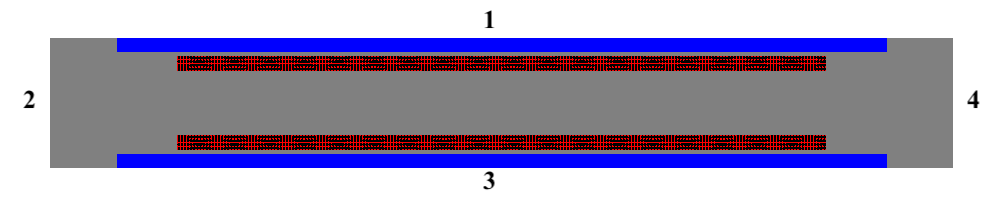
\includegraphics[width=0.85\linewidth]{straightened_slab.png}
    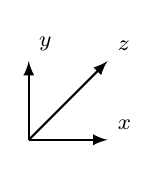
\begin{tikzpicture}
        \draw[ thick,-latex] (0,0) -- (1,0) node[anchor=south west] {$x$};
        \draw[ thick,-latex] (0,0) -- (0,1) node[anchor=south west] {$y$};
        \draw[ thick,-latex] (0,0) -- (1,1) node[anchor=south west] {$z$};
       \tkzText[above](-0.3,-0.7){}
       \end{tikzpicture} 
    \raggedright
    \resizebox{0.3\textwidth}{!}{
        \hspace{1cm}
        \fbox{\begin{tabular}{ll}
            \textcolor{fhrblue}{$\blacksquare$} & FLiBe \\
            \textcolor{fhrgrey}{$\blacksquare$} & Graphite (Fuel Plank)\\
            \textcolor{fhrred}{$\blacksquare$} & Graphite (Fuel Stripe) \\
            \textcolor{fhrblack}{$\blacksquare$} & TRISO particle 

            \end{tabular}}}
    \caption{Straightened \acrfull{AHTR} fuel slab with reflective boundary 
    conditions. Original slanted fuel slabs can be seen in Figures 
    \ref{fig:ahtr-fuel-assembly} and \ref{fig:ahtr-fuel-plank}.}
    \label{fig:straightened_slab}
\end{figure}
The slab has $27.1 \times 3.25 \times 1.85\ cm^3$ dimensions with reflective 
boundary conditions.
I use the same materials as in the \gls{FHR} benchmark (Chapter \ref{chap:fhr-benchmark}), 
except that I homogenized each \gls{TRISO} particle's four outer layers: 
porous carbon buffer, inner pyrolytic carbon, silicon carbide layer, and the 
outer pyrolytic carbon. 
The \gls{TRISO} particle dimensions remain the same.
Table \ref{tab:keff_triso} reports OpenMC's reported $k_{eff}$ for this original 
straightened \gls{AHTR} configuration with and without the outer layer \gls{TRISO} 
homogenization.
\begin{table}[H]
    \centering
    \onehalfspacing
    \caption{Straightened \acrfull{AHTR} fuel slab $k_{eff}$ for case with 
    no \gls{TRISO} homogenization and case with homogenization of the four outer 
    layers. Both simulations were run on one BlueWaters XE Node.}
	\label{tab:keff_triso}
    \footnotesize
    \begin{tabular}{llc}
    \hline 
    \textbf{TRISO Homogenization}& \textbf{$k_{eff}$} & \textbf{Simulation time [s]}  \\
    \hline 
    None & $1.38548 \pm 0.00124$ & 233\\ 
    Four outer layers & $1.38625 \pm 0.00109$ & 168\\ 
    \hline
    \end{tabular}
\end{table}
The \gls{TRISO} particle outer four-layer homogenization resulted in a $30\%$ 
speed-up without compromising accuracy with $k_{eff}$ values within each 
other's uncertainty.


\section{Optimization Problem Definition}
I limited the problem's scope to vary the following \gls{AHTR} parameters: 
\begin{itemize}
    \item \gls{TRISO} particle packing fraction distribution, $\rho_{TRISO}(\vec{r})$
    \item Total fuel packing fraction
    \item \gls{FLiBe} coolant channel shape 
\end{itemize} 
Three reactor optimization objectives were selected to address contrasting 
reactor core qualities. 
Table \ref{tab:objectives} describes the optimization objectives, how I quantified 
them, and the motivation for each.
\begin{table}[H]
    \centering
    \onehalfspacing
    \caption{\acrfull{ROLLO} optimization problem objectives with their quantification 
    descriptions, and motivation.}
	\label{tab:objectives}
    \footnotesize
    \begin{tabular}{p{4cm}p{5cm}p{5cm}}
    \hline 
    \textbf{Objective}& \textbf{Quantification}& \textbf{Motivation} \\
    \hline
    Minimize fuel amount & Minimize total fuel packing fraction & Cost savings, Non-proliferation \\ 
    \hline
    Maximize heat transfer & Minimize maximum temperature & Enable system to perform at a higher power with minimized thermal stress \\
    \hline
    Minimize power peaking & Minimize power peaking factor normalized by fuel distribution & Efficient fuel utilization, longer core life, safety\\
    \hline
    \end{tabular}
\end{table}
% top objectives of any reactor optimization process. 
% explain why each objective is important 
% should explore more optimization objectives, but this is good for 
% the scope of the dissertation
\gls{ROLLO} drives the evolutionary algorithm optimization process. 
\gls{ROLLO} varies the input parameters resulting in different AHTR slab geometries, 
the neutronics and multi-physics of the new geometries are then modeled in the 
OpenMC and Moltres software, these software calculate the problem's objective 
and constraint values. 
\gls{ROLLO} then iterates based on these results to find the 
input parameters that best optimize for the problem's objectives. 
Table \ref{tab:slab-obj-breakdown} shows the details of each \gls{ROLLO} 
optimization problem explored in this chapter.
\begin{table}[H]
    \centering
    \onehalfspacing
    \caption{\acrfull{ROLLO} simulations for optimizing \acrfull{AHTR}
    fuel slab. $PF$: Total Fuel Packing Fraction, $T_{max}$: Maximum Slab Temperature, 
    $PPF$: Normalized Power Peaking Factor, $\rho_{TRISO}(\vec{r})$: 
    \gls{TRISO} particle distribution}
	\label{tab:slab-obj-breakdown}
    \footnotesize
    \begin{tabular}{cllll}
    \hline 
    \textbf{Num Objectives} & \textbf{Objectives} & \textbf{Constraints} &\textbf{Varying Parameters} & \textbf{Simulation Software} \\
    \hline
    1 & \tabitem max($k_{eff}$) & - &\tabitem $\rho_{TRISO}(\vec{r})$ & OpenMC\\
    1 & \tabitem min($PF$) & \tabitem $k_{eff}$ $>$ 1.39 &\tabitem $\rho_{TRISO}(\vec{r})$ & OpenMC \\
      & & & \tabitem $PF$ & \\
    1 & \tabitem min($T_{max}$) & \tabitem $k_{eff}$ $>$ 1.0 &\tabitem $\rho_{TRISO}(\vec{r})$ & OpenMC, Moltres\\
    1 & \tabitem min($PPF$) & \tabitem $k_{eff}$ $>$ 1.0 &\tabitem $\rho_{TRISO}(\vec{r})$ & OpenMC\\
    1 & \tabitem min($PF$) & \tabitem $k_{eff}$ $>$ 1.39 &\tabitem FLiBe channel shape & OpenMC \\
      & & & \tabitem $PF$ & \\
    1 & \tabitem min($T_{max}$) & \tabitem $k_{eff}$ $>$ 1.0 &\tabitem FLiBe channel shape & OpenMC, Moltres\\
    1 & \tabitem min($PPF$) & \tabitem $k_{eff}$ $>$ 1.0 &\tabitem FLiBe channel shape & OpenMC\\
    \hline
    2 & \tabitem min($PF$) & $k_{eff}$ $>$ 1.39 & \tabitem $\rho_{TRISO}(\vec{r})$ & OpenMC, Moltres\\
      & \tabitem min($T_{max}$) & & \tabitem $PF$ & \\
    2 & \tabitem min($PF$) & $k_{eff}$ $>$ 1.39 & \tabitem $\rho_{TRISO}(\vec{r})$ & OpenMC\\
      & \tabitem min($PPF$) & & \tabitem $PF$ & \\
    2 & \tabitem min($T_{max}$) & $k_{eff}$ $>$ 1.0 & \tabitem $\rho_{TRISO}(\vec{r})$ & OpenMC, Moltres\\
      & \tabitem min($PPF$) & & & \\
    \hline
    3 & \tabitem min($PF$) & $k_{eff}$ $>$ 1.39 & \tabitem $\rho_{TRISO}(\vec{r})$ & OpenMC, Moltres\\
    & \tabitem min($PPF$) & & \tabitem $PF$ & \\
      & \tabitem min($T_{max}$) & & & \\
    \hline
    \end{tabular}
\end{table}

\section{AHTR Slab Modeling}
In this section, I describe the AHTR slab modeling workflow: from the AHTR geometry 
variation input parameters, to the OpenMC and Moltres models, and finally the 
output and constraint values. 
Figure \ref{fig:ahtr-slab-flow} illustrates the modeling workflow. 
\begin{figure}[H]
    \centering
    \begin{tikzpicture}[node distance=0.5cm]
        \tikzstyle{every node}=[font=\footnotesize]
        \node (1) [e72block] {\textit{Total PF}};
        \node (2) [b72block, right=of 1] {\textbf{PF}};
        \node (3) [e72block, above=of 2] {Input Parameters};
        \node (4) [e72block, below=of 1] {$\rho_{TRISO}(\vec{r})$};
        \node (5) [b72block, right=of 4] {\textbf{a, b, c}};
        \node (6) [e72block, below=of 4] {FliBE Coolant Channel Shape};
        \node (7) [b72block, right=of 6] {?};
        \node (8) [o72block, right=of 2, xshift=0.8cm, yshift=0.5cm] {OpenMC Model};
        \node (9) [e72block, above=of 8] {Input Files};
        \node (10) [o72block, right=of 5, xshift=0.8cm] {Group Constants};
        \node (11) [o72block, right=of 7, xshift=0.8cm, yshift=-0.5cm] {Moltres Model};
        \node (12) [b72block, right=of 8, xshift=0.8cm, yshift=0.8cm] {$k_{eff}$}; 
        \node (13) [e72block, above=of 12] {Constraints};
        \node (14) [e72block, below=of 12] {Objectives};
        \node (15) [b72block, below=of 14] {PF};
        \node (16) [b72block, below=of 15] {PPF};
        \node (17) [b72block, below=of 16] {$T_{max}$};
        \draw [arrow] (2) -- ([shift={(0cm,0cm)}]2.east) -- ([shift={(0cm,0cm)}]8.west);
        \draw [arrow] (5) -- ([shift={(0cm,0cm)}]5.east) -- ([shift={(0cm,0cm)}]8.west);
        \draw [arrow] (7) -- ([shift={(0cm,0cm)}]7.east) -- ([shift={(0cm,0cm)}]8.west);
        \draw [arrow] (8) -- ([shift={(0cm,0cm)}]8.south) -- node[anchor=west] {generates} ([shift={(0cm,0cm)}]10.north);
        \draw [arrow] (10) -- ([shift={(0cm,0cm)}]10.south) -- node[anchor=west] {input into} ([shift={(0cm,0cm)}]11.north);
        \draw [arrow] (8) -- ([shift={(0cm,0cm)}]8.east) -- ([shift={(0cm,0cm)}]12.west);
        \draw [arrow] (8) -- ([shift={(0cm,0cm)}]8.east) -- ([shift={(0cm,0cm)}]15.west);
        \draw [arrow] (8) -- ([shift={(0cm,0cm)}]8.east) -- ([shift={(0cm,0cm)}]16.west);
        \draw [arrow] (11) -- ([shift={(0cm,0cm)}]11.east) -- ([shift={(0cm,0cm)}]17.west);
    \end{tikzpicture}
    \caption{\acrfull{AHTR} fuel slab modeling workflow.} 
    \label{fig:ahtr-slab-flow}
\end{figure}

\subsection{Input Parameter Modeling}
In this section, I describe how I modeled the \gls{AHTR} input
parameter variations: total fuel packing fraction, TRISO particle packing fraction 
distribution, and \gls{FLiBe} coolant channel shape. 
The total fuel packing fraction is a single numerical input.

I vary the TRISO particle packing fraction across the fuel slab by dividing the 
slab into ten cells along the x-axis between the \gls{FLiBe} and graphite 
buffers, resulting in ten $2.31 \times 2.55 \times 1.85\ cm^3$ cells, and varying
the packing fraction in each cell.
A sine distribution governs the \gls{TRISO} particle packing fraction's 
distribution across cells:
\begin{align}
    PF(x) &= \left(a\cdot sin(b\cdot x + c) + 2\right) \cdot NF\\
    \intertext{where}
    PF &= \mbox{packing fraction } [-] \nonumber \\ 
    a &= \mbox{amplitude, peak deviation of the function from zero } [-] \nonumber \\
    b &= \mbox{angular frequency, rate of change of the function argument } [\frac{radians}{cm}] \nonumber \\
    c &= \mbox{phase, the position in its cycle the oscillation is at t = 0 } [radians]\nonumber \\
    x &= \mbox{midpoint value for each cell } [cm]\nonumber \\
    NF &= \mbox{Normalization factor } [-]\nonumber
\end{align}
The normalization factor ensures the correct total packing fraction 
in the slab regardless the \gls{TRISO} particle distribution.
I use OpenMC's \texttt{pack\_spheres} function to randomly disperse the calculated packing 
fraction in each fuel slab slice. 
For example, a total packing fraction of 0.0979, and packing fraction distribution of 
$PF(x) = \left(0.5\cdot sin(\frac{\pi}{3}\cdot x + \pi) + 2\right)  \cdot NF$, 
results in the following packing fractions for the ten cells: 0.103, 0.120, 
0.049, 0.138, 0.076, 0.081, 0.136, 0.048, 0.125, and 0.098. 
Figure \ref{fig:triso_distribution} shows this sine distribution, highlights 
the packing fraction at the respective midpoints, and displays the slab's x-y 
axis view with packing fraction varying based on this sine distribution. 
\begin{figure}[H]
    \centering
    \makebox[\textwidth][c]{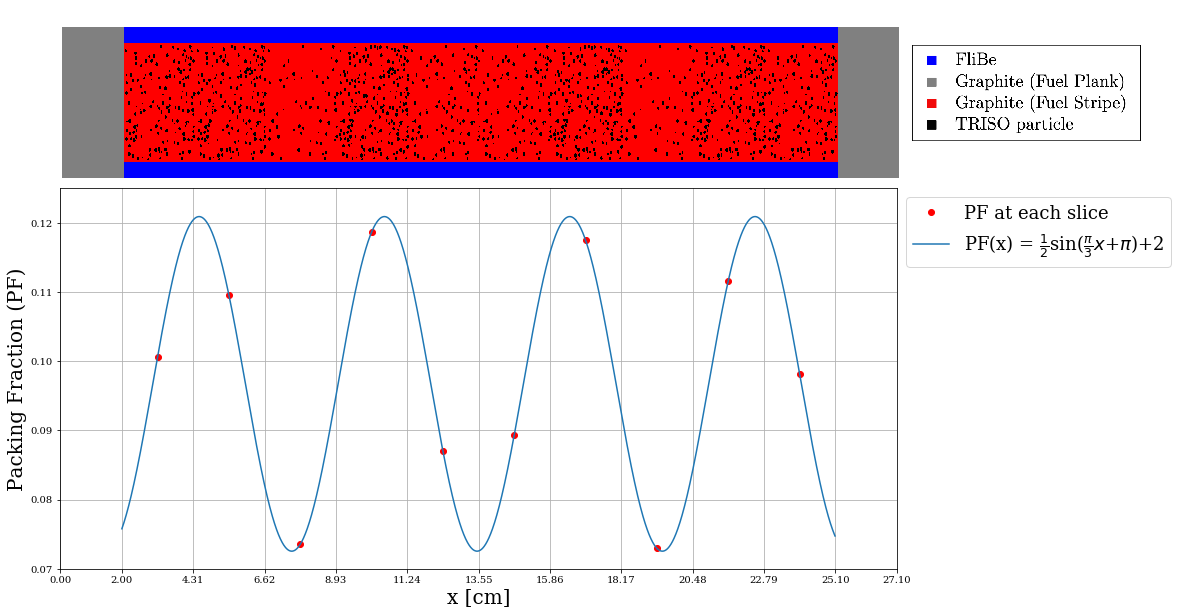
\includegraphics[width=1.1\linewidth]{triso_distribution_sine.png}} 
    \caption{Above: Straightened \acrfull{AHTR} fuel slab with varying \gls{TRISO} particle 
    distribution across ten cells based on the sine distribution. 
    Below: $PF(x) = (0.5\ sin(\frac{\pi}{3}x + \pi) + 2)  \times NF$ 
    sine distribution with red points indicating the packing fraction at each cell. }
    \label{fig:triso_distribution}
\end{figure}
Thus, ROLLO will vary $a, b, c$ constants to find an optimal TRISO particle 
sine distribution. 

%% DESCRIPTION FOR COOLANT CHANNEL SHAPE DEFINITION.
I vary the FliBE coolant channel shape by: ...

\subsection{AHTR Slab OpenMC and Moltres Models}
\label{sec:ahtr-moltres-hom}
The input parameter modeling outlined in the previous section are inputs into 
the OpenMC neutronics model. 
The total packing fraction, TRISO particle distribution, and FliBE coolant 
channel shape are reflected in the OpenMC input file. 
Thus, there is TRISO level fidelity in the OpenMC neutronics model. 
The OpenMC neutronics model outputs the $k_{eff}$ constraint value, and the 
total packing fraction, and normalized power peaking factor output values. 
Section \ref{sec:ahtr_slab_output} gives further description of calculation for 
each output and constraint parameter.

For the Moltres model, a TRISO-level fidelity mesh file is impractical 
and will result in an extremely long Moltres runtimes. 
Moltres accepts group constant data from OpenMC for the Moltres multigroup 
neutron diffusion calculations and a mesh file representing the reactor geometry. 
Thus, for a successful \gls{AHTR} Moltres simulation, I established 
suitable spatial and energy homogenization that preserves accuracy while 
maintaining an acceptable runtime.

For spatial homogenization of the straightened \gls{AHTR} fuel slab, I used 
OpenMC's \textit{cell} domain type to compute multigroup cross sections for 
different \textit{cells}. 
I discretized the slab into 13 \textit{cells}: FLiBe, left graphite, right 
graphite, and ten fuel cells (each cell has a different packing fraction). 
Figure \ref{fig:straightened_slab_mg} illustrates the \gls{AHTR} spatial 
homogenization for the OpenMC multigroup calculation. 
\begin{figure}[H]
    \centering
    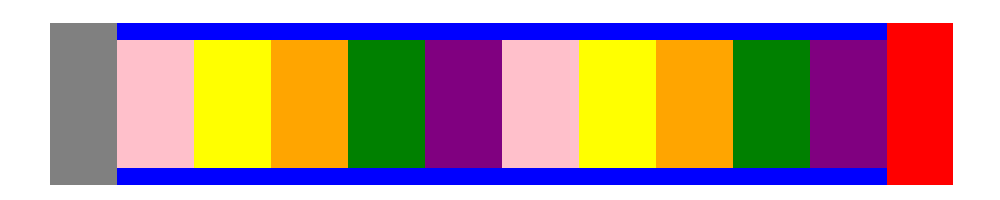
\includegraphics[width=\linewidth]{straightened_slab_mg.png}
    \raggedright
    \resizebox{0.5\textwidth}{!}{
        \hspace{1cm}
        \fbox{\begin{tabular}{llll}
            \textcolor{fhrblue}{$\blacksquare$} & FLiBe & 
            \textcolor{fhrgrey}{$\blacksquare$} & Left Graphite \\
            \textcolor{fhrred}{$\blacksquare$} & Right Graphite &
            \textcolor{fhrpink}{$\blacksquare$} & Fuel cell 1/6 \\
            \textcolor{fhryellow}{$\blacksquare$} & Fuel cell 2/7 &
            \textcolor{fhrorange}{$\blacksquare$} & Fuel cell 3/8 \\
            \textcolor{fhrgreen}{$\blacksquare$} & Fuel cell 4/9 &
            \textcolor{fhrpurple}{$\blacksquare$} & Fuel cell 5/10 \\
            \end{tabular}}}
    \caption{Straightened \acrfull{AHTR} fuel slab spatially discretized into 
    13 \textit{cells} for OpenMC multigroup calculation.}
    \label{fig:straightened_slab_mg}
\end{figure}
I used the four group energy structure derived by Gentry et al. 
\cite{gentry_development_2016} for \gls{AHTR} geometries. 
Table \ref{tab:energy_structures} defines the group boundaries. 
\begin{table}[H]
    \centering
    \onehalfspacing
    \caption{4-group energy structures for \acrfull{AHTR} geometry 
    derived by \cite{gentry_development_2016}.}
	\label{tab:energy_structures}
    \footnotesize
    \begin{tabular}{lll}
    \hline
    \multicolumn{3}{c}{\textbf{Group Boundaries [MeV]}} \\ 
    \hline
    \textbf{Group $\#$}& \textbf{Upper Bound} & \textbf{Lower Bound}  \\
    \hline 
    1 & $2.0000\times 10^1$ & $9.1188\times 10^{-3}$ \\ 
    2 & $9.1188\times 10^{-3}$ & $2.9023\times 10^{-5}$\\
    3 & $2.9023\times 10^{-5}$ & $1.8554\times 10^{-6}$\\
    4 & $1.8554\times 10^{-6}$ & $1.0000\times 10^{-12}$\\
    \hline
    \end{tabular}
\end{table}

To ensure that the spatial and energy homogenization preserves accuracy, I 
compared key neutronics parameters for the continuous OpenMC and multigroup 
Moltres simulations.

\subsection{Moltres Model Neutronics Performance Verification}
In this section, I set up a criticality eigenvalue problem in Moltres to demonstrate  
it's ability to reproduce key neutronics parameters using multi-group constant 
data from OpenMC for the AHTR slab.  
The accuracy from this neutronics verification step gives confidence for 
subsequent AHTR slab multiphysics simulations with Moltres. 

% move this to lit review for Moltres
Moltres solves the four-group diffusion equations as a steady-state eigenvalue 
problem to find $k_{eff}$ for the static AHTR slab model: 
\begin{align}
    \frac{1}{v_g} \frac{\partial \phi_g}{\partial t} &= \nabla \cdot D_g
    \nabla \phi_g - \Sigma^r_g \phi_g +
    \sum^G_{g' \neq g} \Sigma^s_{g' \rightarrow g} \phi_{g'} + \chi^p_g
    \sum^G_{g'=1} (1-\beta) \nu \Sigma^f_{g'} \phi_{g'} + \chi^d_g \sum^I_i
    \lambda_i C_i
\end{align}

I will be comparing the key neutronics parameters between two simulations:
\begin{enumerate}
    \item OpenMC simulation with continuous energy and TRISO-level spatial fidelity 
    \item Moltres simulation with 4-group energy and 13-cell spatial homogenization
\end{enumerate}
I outlined the spatially homogenization used in section ??. 
The OpenMC simulation with TRISO-level fidelity generates the group 
constants for the energy and spatially homogenized Moltres simulation. 

% Describe how you calculated each simulation. MGXS generation and group 
% constant generation

% say i changed it to reflective and temperature = 948K

\subsubsection{Effective Multiplication Factor}
In this section, I include results from a homogenized OpenMC simulation as well to 
distinguish between differences caused by spatial homogenization, and differing 
OpenMC and Moltres normalization and solving methods. 
% explain how this works 
\begin{table}[H]
    \centering
    \onehalfspacing
    \caption{AHTR Fuel Slab's $k_{eff}$ values from OpenMC and Moltres at 948K.
    Normalized difference is the pcm difference normalized by $k_{eff}$}
	\label{tab:keff_ahtr_moltres}
    \footnotesize
    \begin{tabular}{lllcc}
    \hline 
    \textbf{Software}& \textbf{Homogenized?}& \textbf{$k_{eff}$} & \textbf{Difference [pcm]}  
    & \textbf{Normalized Difference [pcm]}\\
    \hline 
    OpenMC & No & $1.41402 \pm 0.00140$ & - & -\\ 
    OpenMC & Yes & $1.41473 \pm 0.00098$ & +71 & -\\ 
    Moltres & Yes & $1.40696 $ & -706 & -502\\ 
    \hline
    \end{tabular}
\end{table}
The 71pcm $k_{eff}$ difference between continuous and homogenized OpenMC 
simulations show that the selected spatial and energy homogenizations
are acceptable. 
However, there is a 502pcm difference in the Moltres simulation's $k_{eff}$.
Possible reasons are that the neutron diffusion method used in Moltres does not 
approximate this reactor geometry as well. 
The diffusion coefficients for this reactor type are approximately 1cm. 
The FliBE coolant channel has a 0.35cm width which is smaller than the diffusion
coefficient, resulting in poor approximations. 

\subsubsection{Reactivity Coefficients}
Moltres' delayed neutron fraction, $\beta{eff}$, is calculated by taking the 
normalized difference between $k_{eff}$ values with and without DNPs. 
The  $\beta{eff}$ values from OpenMC and Moltres show excellent 
agreement with a discrepancy of 0.1pcm. 
\begin{table}[H]
    \centering
    \onehalfspacing
    \caption{AHTR Fuel Slab's $\beta_{eff}$ values from OpenMC and Moltres at 948K.}
	\label{tab:betaeff_ahtr_moltres}
    \footnotesize
    \begin{tabular}{lllc}
    \hline 
    \textbf{Software}& \textbf{Homogenized?}& \textbf{$\beta_{eff}$ [pcm]} 
    & \textbf{Difference [pcm]}  \\
    \hline 
    OpenMC & No &  654.3 & - \\ 
    Moltres & Yes & 654.4 & 0.1\\ 
    \hline
    \end{tabular}
\end{table}
I calculated the temperature reactivity coefficients with equation ??. % FHR BM section
Temperature reactivity feedback arises mainly from Doppler broadening of 
resonance absorption peaks and thermal expansion.
The total temperature coefficients from OpenMC and Moltres show good 
agreement with a discrepancy of 0.4 pcm/K.
\begin{table}[H]
    \centering
    \onehalfspacing
    \caption{AHTR Fuel Slab's total reactivity coefficient values calculated from 
    OpenMC and Moltres at 948K and 1100K.}
	\label{tab:reactivity_ahtr_moltres}
    \footnotesize
    \begin{tabular}{lllc}
    \hline 
    \textbf{Software}& \textbf{Homogenized?}& \textbf{Total $\frac{\Delta \rho}{\Delta T}$ [pcm/K]} 
    & \textbf{Difference [pcm/K]}  \\
    \hline 
    OpenMC & No &  -8.4 & - \\ 
    Moltres & Yes & -8.8 & -0.4\\ 
    \hline
    \end{tabular}
\end{table}

\subsubsection{Flux Distribution}
Moltres' source term ($Q_f$) is defined by: 
\begin{align}
\label{eq:moltres-source-term}
    Q_f &= \sum_{g=1}^G \epsilon_{f,g}\Sigma_{f,g}\phi_g
\intertext{where} 
Q_f &= \mbox{source term } [\frac{MeV}{cm^3s}] \nonumber \\
G &= \mbox{number of discrete groups, g } [-] \nonumber \\
\epsilon_{f,g} &= \mbox{heat produced per fission } [MeV] \nonumber \\
\Sigma_{f,g} &= \mbox{macroscopic cross section for fission due to neutrons in group g } [\frac{1}{cm}] \nonumber \\
\phi_g &= \mbox{flux of neutrons in group g } [\frac{n}{cm^2s}]\nonumber
\end{align}
The $\epsilon_{f,g}$ and $\Sigma_{f,g}$ terms are provided to Moltres through 
the group constants generated by neutronics software, OpenMC.
Thus, differences in the source term between OpenMC and Moltres are dependent on 
the flux. 
Comparison of flux distributions produced by Moltres and OpenMC are key to 
ensuring that temperature distribution is accurately calculated in Moltres.

Figure \ref{fig:flux_948K} shows the 4-group flux distributions for OpenMC and 
Moltres. 
\begin{figure}[H]
    \centering
    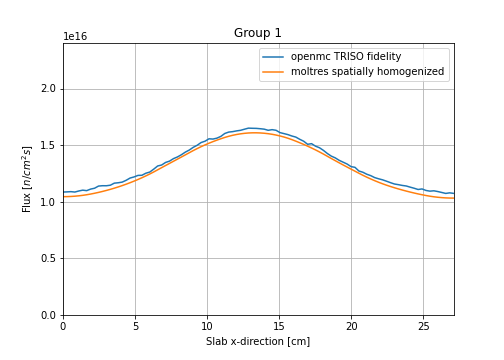
\includegraphics[width=0.48\linewidth]{flux_group1_948K.png} 
    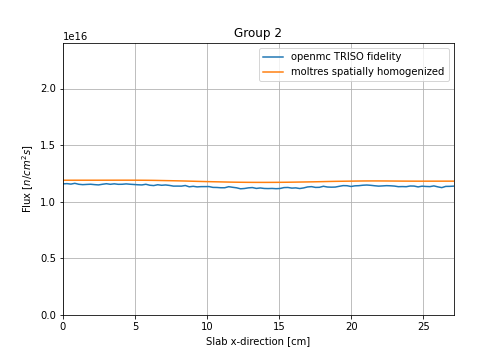
\includegraphics[width=0.48\linewidth]{flux_group2_948K.png} 
    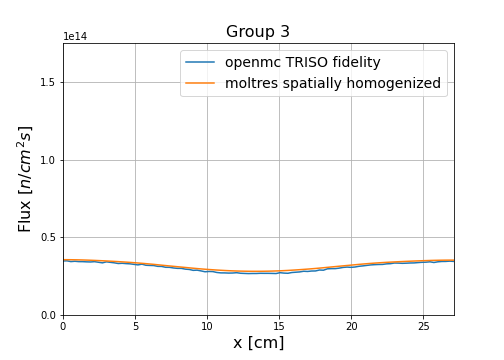
\includegraphics[width=0.48\linewidth]{flux_group3_948K.png} 
    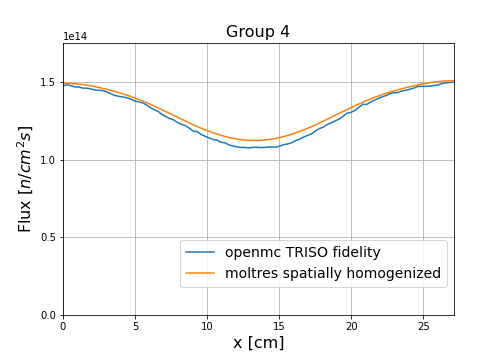
\includegraphics[width=0.48\linewidth]{flux_group4_948K.png} 
    \caption{AHTR fuel slab's centerline neutron flux distribution in 4 groups
    at 948K. 
    Energy Group 1: E $> 9.1188 \times 10^{-3}$ MeV, 
    Energy Group 2: $2.9023 \times 10^{-5} < E < 9.1188 \times 10^{-3}$ MeV,
    Energy Group 3:  $1.8556 \times 10^{-5} < E < 2.9023 \times 10^{-5}$ MeV,
    Energy Group 4:  $1.0 \times 10^{-12} < E < 1.8554 \times 10^{-6}$ MeV}
    \label{fig:flux_948K}
\end{figure}
The OpenMC simulation shows higher flux in Group 1, and lower flux in the
Group 2 and Group 3. 
However, there is an overall good agreement for each group's flux.  

\subsubsection{Neutron Energy Spectrum}
Figure \ref{fig:neutron_spectrum_948K} shows the neutron spectrum the OpenMC simulation 
for both 252 and 4 , and 4-group Moltres simulation. 

 \begin{figure}[H]
    \centering
    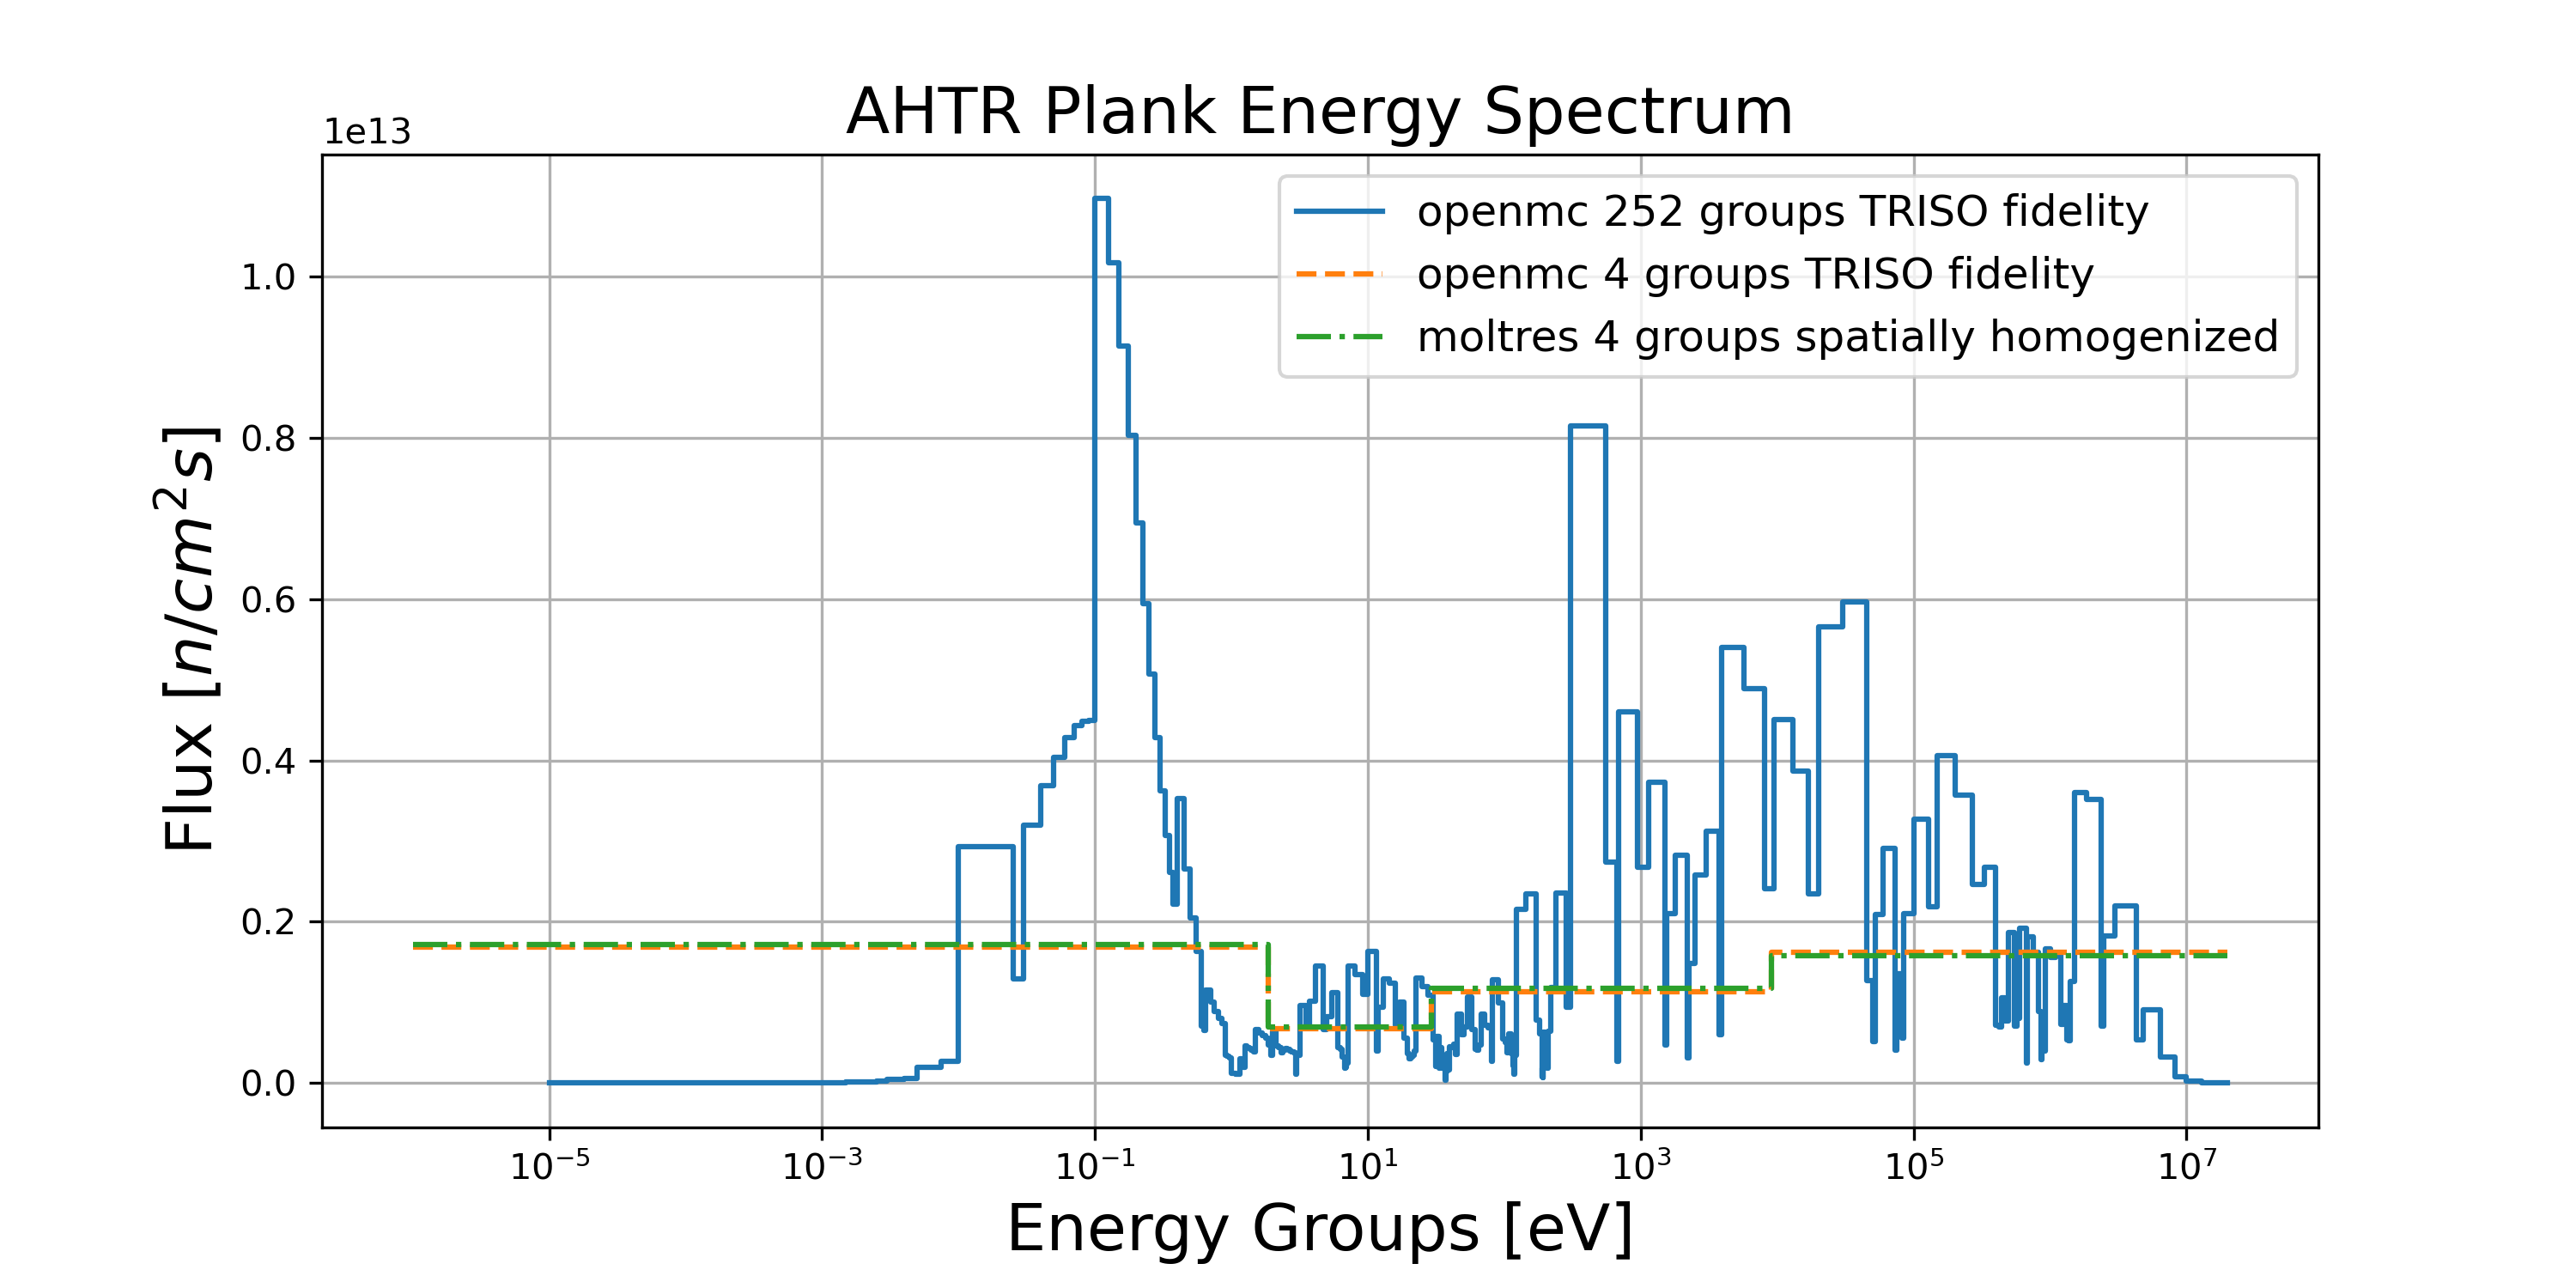
\includegraphics[width=\linewidth]{neutron_spectrum_948K.png}
    \caption{AHTR fuel slab's neutron spectrum.}  
    \label{fig:neutron_spectrum_948K}
\end{figure}

In summary, Moltres replicated the relevant neutronics parameters accurately 
using group constant data from OpenMC. % more description

\subsection{Moltres AHTR Steady-State Temperature Model}
\label{sec:ahtr-moltres-model}
% how to model heat transfer for constant coolant channel shape and varying shape 
One of the ROLLO AHTR optimization objectives is minimizing the maximum 
temperature in the slab. 
A neutronics simulation cannot calculate maximum temperature; thus, I introduced 
AHTR slab temperature modeling with Moltres.
I used OpenMC to generate multigroup neutronics data for the AHTR slab at 948K 
for four energy groups and eight precursor groups based on the spatial and 
energy homogenization described in section \ref{sec:ahtr-moltres-hom}.
The Moltres AHTR Steady-State Temperature Model first solves for the neutronics 
in slab and uses that to solve for the temperature distribution in the slab 
for a defined power. 
The temperature model assumes conductive heat transfer throughout the domain 
and heat removal by uniform salt flow in the coolant region. 
These assumptions ignore flow and turbulent effects that would most likely be 
present. 
However, an in-depth AHTR Moltres model that includes turbulence model is 
out of scope for this dissertation. 

Equation \ref{eq:moltres-temp} described Moltres' governing equation for 
temperature.
In the 2D cross-sectional AHTR Steady-State Temperature Model, I ignore the 
time-dependent and velocity-dependent terms since I am solving for steady-state 
and there is no moving fuel: 
\begin{align}
    - \nabla \cdot (k_i \nabla T) &= Q_i
\intertext{where:}
k_i &= \mbox{thermal conductivity of material i} \nonumber \\
T &= \mbox{temperature in the slab} \nonumber \\
Q_i &= \mbox{source or sink term in material i} \nonumber
\end{align} 
I use insulated temperature boundary conditions.  
Table \ref{tab:ahtr-thermal-conducitivity} shows the thermal conductivity values 
used for each AHTR slab material. 
\begin{table}[H]
    \centering
    \onehalfspacing
    \caption{AHTR Fuel Slab materials' thermal conductivity.}
	\label{tab:ahtr-thermal-conducitivity}
    \footnotesize
    \begin{tabular}{lp{4cm}l}
    \hline 
    \textbf{Material}& \textbf{Thermal Conductivity [$Wcm^{-1}K^{-1}$]}& \textbf{References} \\ 
    \hline 
    FliBE & 0.01 & \\
    Graphite  & 0.15 & \\
    Fuel  & 0.099 & \\
    \hline
    \end{tabular}
\end{table}
Equation \ref{eq:moltres-source-term} defines the fuel cells' fission source term.
Equation \ref{eq:moltres-heat-removal} defines the heat removal from the AHTR 
fuel slab in the coolant areas: 
\begin{align}
    \label{eq:moltres-heat-removal}
    Q &= h \cdot (T(\vec{r})-T_{ref})
\intertext{where:}
Q &= \mbox{heat removal rate for 1cm thin slice of AHTR slab [W/cm]} \nonumber \\
h &= \mbox{heat transfer coefficient } [\frac{W}{cm \cdot K}] \nonumber \\
T(\vec{r}) &= \mbox{temperature at point $\vec{r}$ [K]} \nonumber \\
T_{ref} &= \mbox{reference temperature [K]} \nonumber
\end{align}

Table \ref{tab:heat-exchanger-constants} shows the values used for 
reference temperature and heat transfer coefficient for the convective 
heat transfer process.
\begin{table}[H]
    \centering
    \onehalfspacing
    \caption{AHTR Fuel Slab's heat transfer constants.}
	\label{tab:heat-exchanger-constants}
    \footnotesize
    \begin{tabular}{llll}
    \hline 
    \textbf{Constant}& \textbf{Value}& \textbf{Units} & \textbf{Notes} \\
    \hline 
    h & 990 & $\frac{W}{cm \cdot K}$ & Calculated in Eq. \ref{eq:calc-htc} \\
    $T_{ref}$ & 923 & K & AHTR Inlet Temperature \\ %cite ahtr 923K inlet temp 
    \hline
    \end{tabular}
\end{table} 
I calculated the heat transfer coefficient ($h$) using Equation \ref{eq:calc-htc} 
for the 1cm-thick AHTR $\Delta z$ slice with the following assumptions: 
\begin{itemize}
    \item it generates a constant amount of power, all of which is removed 
    by the coolant
    \item heat removal occurs at the coolant areas
    \item temperature increase per 1cm slice is constant from the inlet to the 
    outlet 
\end{itemize} 
\begin{align}
    \label{eq:calc-htc}
    h &= \frac{P_{dz}}{A_{coolant}} \div \frac{T_{total}}{H} \\
      &= \frac{1456 W}{23.1 * 0.5 * 2 cm^2} / (50 K / 550 cm) \nonumber \\
      &= 990 W cm^{-1}K^{-1} \nonumber 
\intertext{where:}
h &= \mbox{heat transfer coefficient } [\frac{W}{cm \cdot K}] \nonumber \\
P_{dz} &= \mbox{power produced in 1cm AHTR slab dz slice [$W$]}\nonumber \\
A_{coolant} &= \mbox{cross-sectional coolant area in AHTR slab [$cm^2$]} \nonumber \\
T_{total} &= \mbox{total temperature change from inlet to outlet [$K$]} \nonumber \\
H &= \mbox{AHTR height from inlet to outlet [$cm$]} \nonumber 
\end{align}
In the ROLLO optimization simulations, I vary the FliBE coolant channel shape. 
During the shape variation, I hold the coolant area constant. 
Therefore, the Moltres temperature model holds the heat transfer coefficient ($h$)
constant for all the simulations.  

Using the described models and assumptions, I set up a Moltres AHTR steady-state 
temperature model for a slab with a constant packing fraction of 0.0979 across ten 
fuel cells. 
The \texttt{constant$\_$0.0979} directory in the \texttt{2022-chee-dissertation} 
Github repository contains the model. % cite DOI   
Figure \ref{fig:ahtr_constant_temp} shows the Moltres-generated temperature 
distribution with an average and maximum temperature of 1019K and 1128K, 
respectively.
\begin{figure}[H]
    \centering
    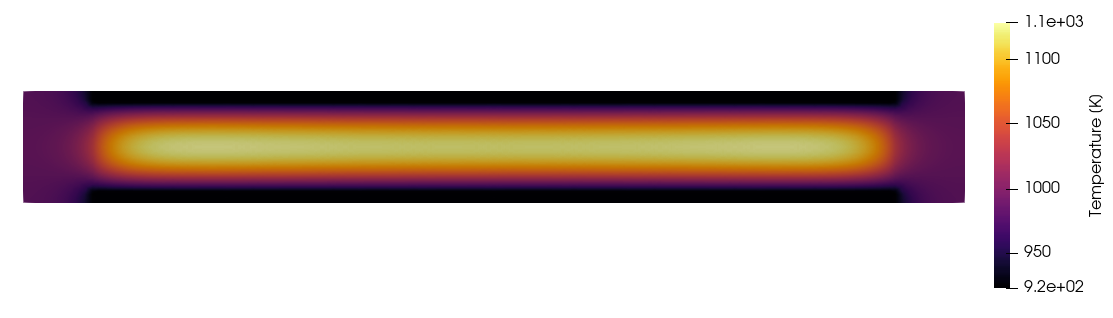
\includegraphics[width=\linewidth]{ahtr_constant_temp.png}
    \caption{AHTR fuel slab's Moltres generated temperature distribution for a 
    slab with a constant packing fraction of 0.0979 across ten fuel cells.}  
    \label{fig:ahtr_constant_temp}
\end{figure}
The temperature distribution is consistent with previous temperature models of 
the AHTR fuel slabs that report an average fuel kernel temperature of 1125K 
\cite{ramey_methodology_2021}. 
Model differences include that Ramey \cite{ramey_methodology_2021} utilized a 
1D temperature model with the original 4-layer TRISO model from the FHR benchmark 
(Figure \ref{fig:straightened_slab}).
This model is 2D and randomly disperses TRISO particles throughout the 
slab while keeping the same overall packing fraction. 
Chapter \ref{chap:fhr-multiphysics-model} conducts a more accurate one-for-one 
comparison \ref{chap:fhr-multiphysics-model}.

% Discuss convergence of Moltres temperature model 

\subsection{Output Parameter Calculation}
\label{sec:ahtr_slab_output}
% PF, Max temp, PPF 
This section describes how I tallied the AHTR model outputs for the ROLLO 
optimization problem objectives (as described in Table \ref{tab:objectives}):
total fuel packing fraction, the maximum temperature in the slab, and 
normalized power peaking factor.  

ROLLO will automatically return the total fuel packing fraction output parameter, 
since it is also an input parameter. 
In the Moltres AHTR slab model, I defined a post processor object to return the 
maximum temperature in the slab. 

To ensure efficient fuel utilization, one of the objectives is to minimize 
fuel-normalized power peaking in the slab, that takes into account fuel amount 
variations across the slab.
I discretized the fuel cell area of the slab into 10 $\times$ 5 blocks, and 
use OpenMC to tally the fission energy production rate (\texttt{fission-q-recoverable}
$[eV/src]$) in each section.
I did not normalize the score to calculate power since the final PPF value is a 
ratio.
% why fission q recoverable
The normalized power peaking factor is calculated: 
\begin{align}
    PPF &= max(\frac{fqr_j}{PF_j}) \div ave(\frac{fqr_j}{PF_j})
\intertext{where}
j &= \mbox{discretized fuel area j} \nonumber \\
PPF &= \mbox{fuel-normalized power peaking factor} \nonumber \\
fqr_j &= \mbox{fission-q-recoverable at position j} \nonumber \\
PF_j &= \mbox{fuel packing fraction at position j} \nonumber
\end{align}

\section{Optimization Results}
In this section, I report the results from the ROLLO optimization simulations 
outlined in Table \ref{tab:slab-obj-breakdown}.
Results from this section can be found in the \texttt{2022-chee-dissertation} 
Github repository under the \texttt{rollo-ahtr-slab} directory. %cite 

\subsection{Single-Objective Optimization}
In this section, I report the results for single objective optimization. 

\subsubsection{Objective: Minimize Total Packing Fraction}
I varied the TRISO particle distribution and total packing fraction, while
constraining $k_{eff} > 1.39$. % why 1.39
Figure \ref{fig:slab-obj-1-pf-evol} shows the total packing fraction evolution and 
figure \ref{fig:slab-obj-1-pf-final} shows the five TRISO particle distributions in 
the final generation with the smallest packing fraction. 
\begin{figure}[]
    \centering
    \begin{subfigure}{\textwidth}
        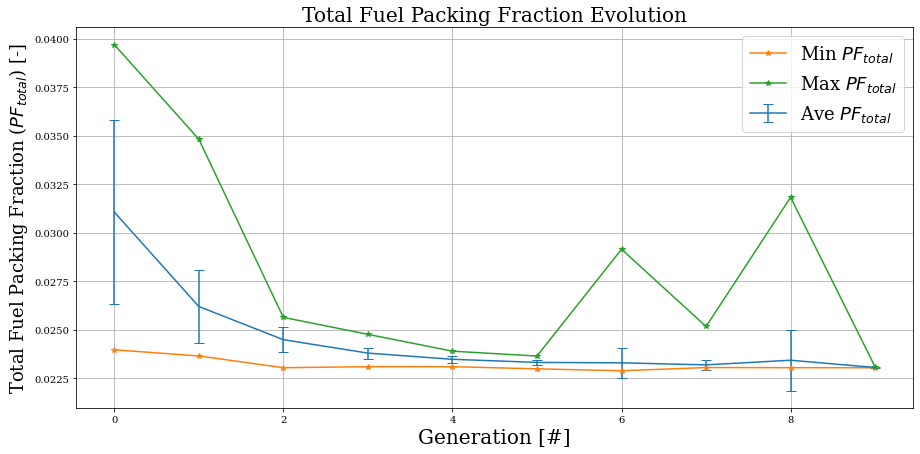
\includegraphics[width=\linewidth]{slab-obj-1-pf-evol.png}
        \caption{Minimum, average, and maximum total packing fraction evolution.}
        \label{fig:slab-obj-1-pf-evol} 
    \end{subfigure}
    \begin{subfigure}{\textwidth}
        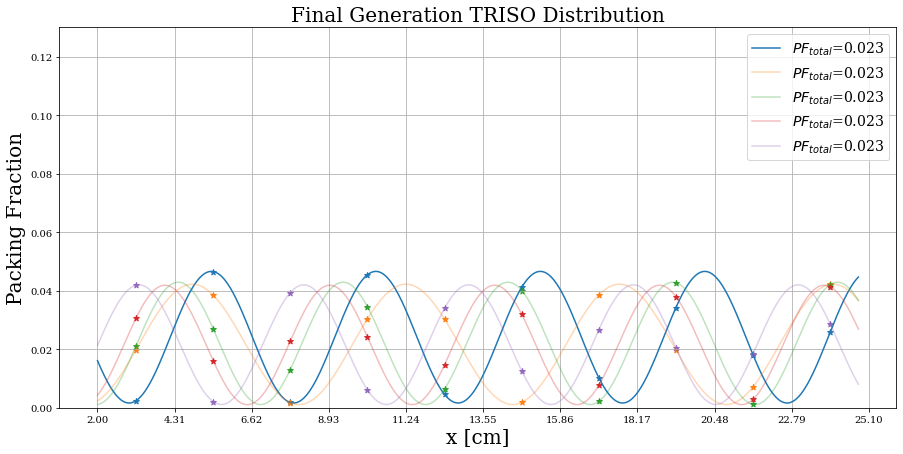
\includegraphics[width=\linewidth]{slab-obj-1-pf-final.png}
        \caption{TRISO particle distribution for the 5 individuals with the 
        smallest packing fraction in generation 9.}
        \label{fig:slab-obj-1-pf-final} 
    \end{subfigure}
    \caption{ROLLO single-objective optimization to minimize total packing fraction. 
    Input parameters varied: total packing fraction, TRISO particle distribution.}
    \label{fig:slab-obj-1-pf}
\end{figure}
The minimum and average packing fractions converged very quickly, as expected 
in this single-objective optimization problem.
By the $9^{th}$ generation, the average, minimum, and maximum packing fraction
values converged to approximately 0.023. 
In figure \ref{fig:slab-obj-1-pf-final}, I observe that the TRISO particle packing 
sine distributions are not exactly the same, but follow a similar pattern of 
alternating between a higher packing fraction, and a lower packing fraction 
in the neighboring fuel cell. 
This up-down fuel packing pattern is to minimize self-shielding effects. 

\subsubsection{Objective: Minimize Maximum Temperature}
I varied the TRISO particle distribution, while constraining $k_{eff} >= 1.0$ and 
total packing fraction of 0.0979 (similar to the FHR benchmark). 
Figure \ref{fig:slab-obj-1-temp-evol} shows the slab's maximum temperature evolution 
and figure \ref{fig:slab-obj-1-temp-final} shows the five TRISO particle 
distributions in the final generation with the lowest maximum temperature.
\begin{figure}[]
    \centering
    \begin{subfigure}{\textwidth}
        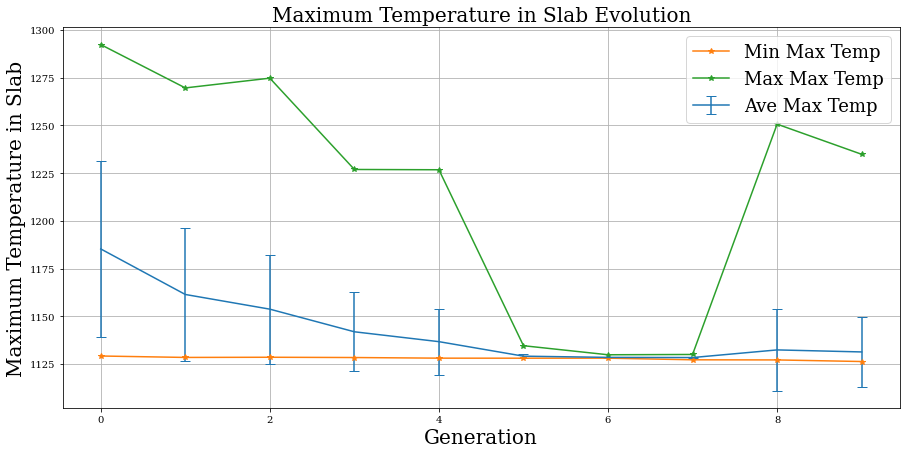
\includegraphics[width=\linewidth]{slab-obj-1-temp-evol.png}
        \caption{Minimum, average, and maximum evolution of maximum temperature in 
        AHTR slab.}
        \label{fig:slab-obj-1-temp-evol} 
    \end{subfigure}
    \begin{subfigure}{\textwidth}
        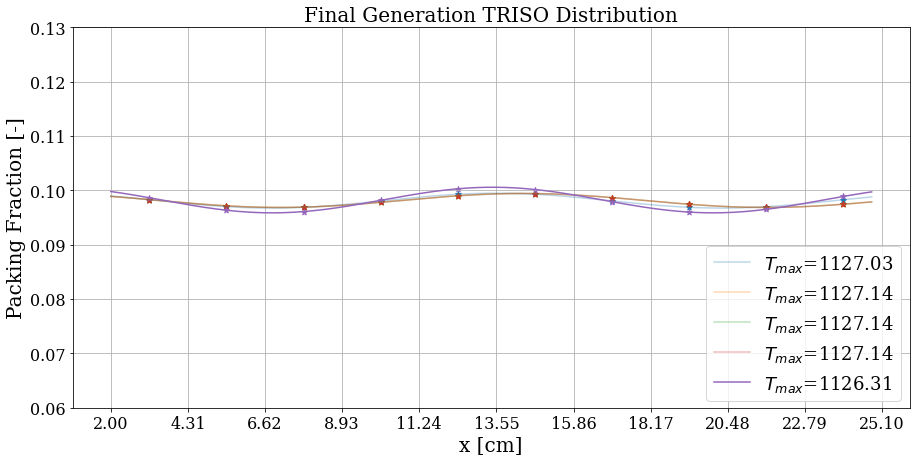
\includegraphics[width=\linewidth]{slab-obj-1-temp-final.png}
        \caption{TRISO particle distribution for the 5 individuals with the 
        lowest maximum temperature in AHTR slab at generation 9.}
        \label{fig:slab-obj-1-temp-final} 
    \end{subfigure}
    \caption{ROLLO single-objective optimization to minimize maximum temperature 
    in the slab. Input parameters varied: TRISO particle distribution.}
    \label{fig:slab-obj-1-temp}
\end{figure}
The minimum and average slab's maximum temperature converged to approximately 
1125 K. 
In figure \ref{fig:slab-obj-1-temp-final}, I observe that a mostly flat TRISO 
particle distribution minimizes maximum temperature in the slab, 
the TRISO particle distribution has two small dips at the one-third and two-third 
points in the slab (6.62cm and 20.48cm). 
A fully flat TRISO particle distribution results in a higher maximum temperature in 
the slab of 1128K, as reported in section \ref{sec:ahtr-moltres-model}. 
Figure \ref{fig:slab-obj-1-temp-distr} shows the temperature distribution 
for the slab with mostly flat and flat TRISO particle distributions.
\begin{figure}[H]
    \centering
    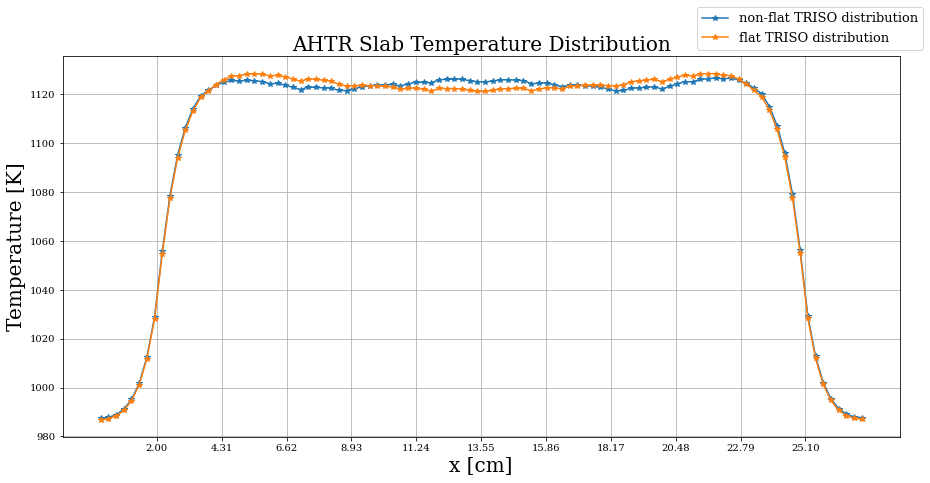
\includegraphics[width=\linewidth]{slab-obj-1-temp-distr.png}
    \caption{}
    \label{fig:slab-obj-1-temp-distr}
\end{figure}
The AHTR slab with a flat TRISO particle distribution has higher slab temperatures 
on the left and right sides near the moderator. 
To combat this temperature peak, ROLLO found a TRISO particle distribution that 
has a slight dip near the moderator regions, resulting in a lower maximum 
temperature.  

\subsubsection{Objective: Minimize Normalized Power Peaking Factor}
I varied the TRISO particle distribution, while constraining $k_{eff} >= 1.0$ and 
total packing fraction of 0.0979 (similar to the FHR benchmark). 
Figure \ref{fig:slab-obj-1-ppf-evol} shows the slab's normalized power peaking 
factor evolution and figure \ref{fig:slab-obj-1-ppf-final} shows the five TRISO particle 
distributions in the final generation with the normalized power peaking factor. 
\begin{figure}[]
    \centering
    \begin{subfigure}{\textwidth}
        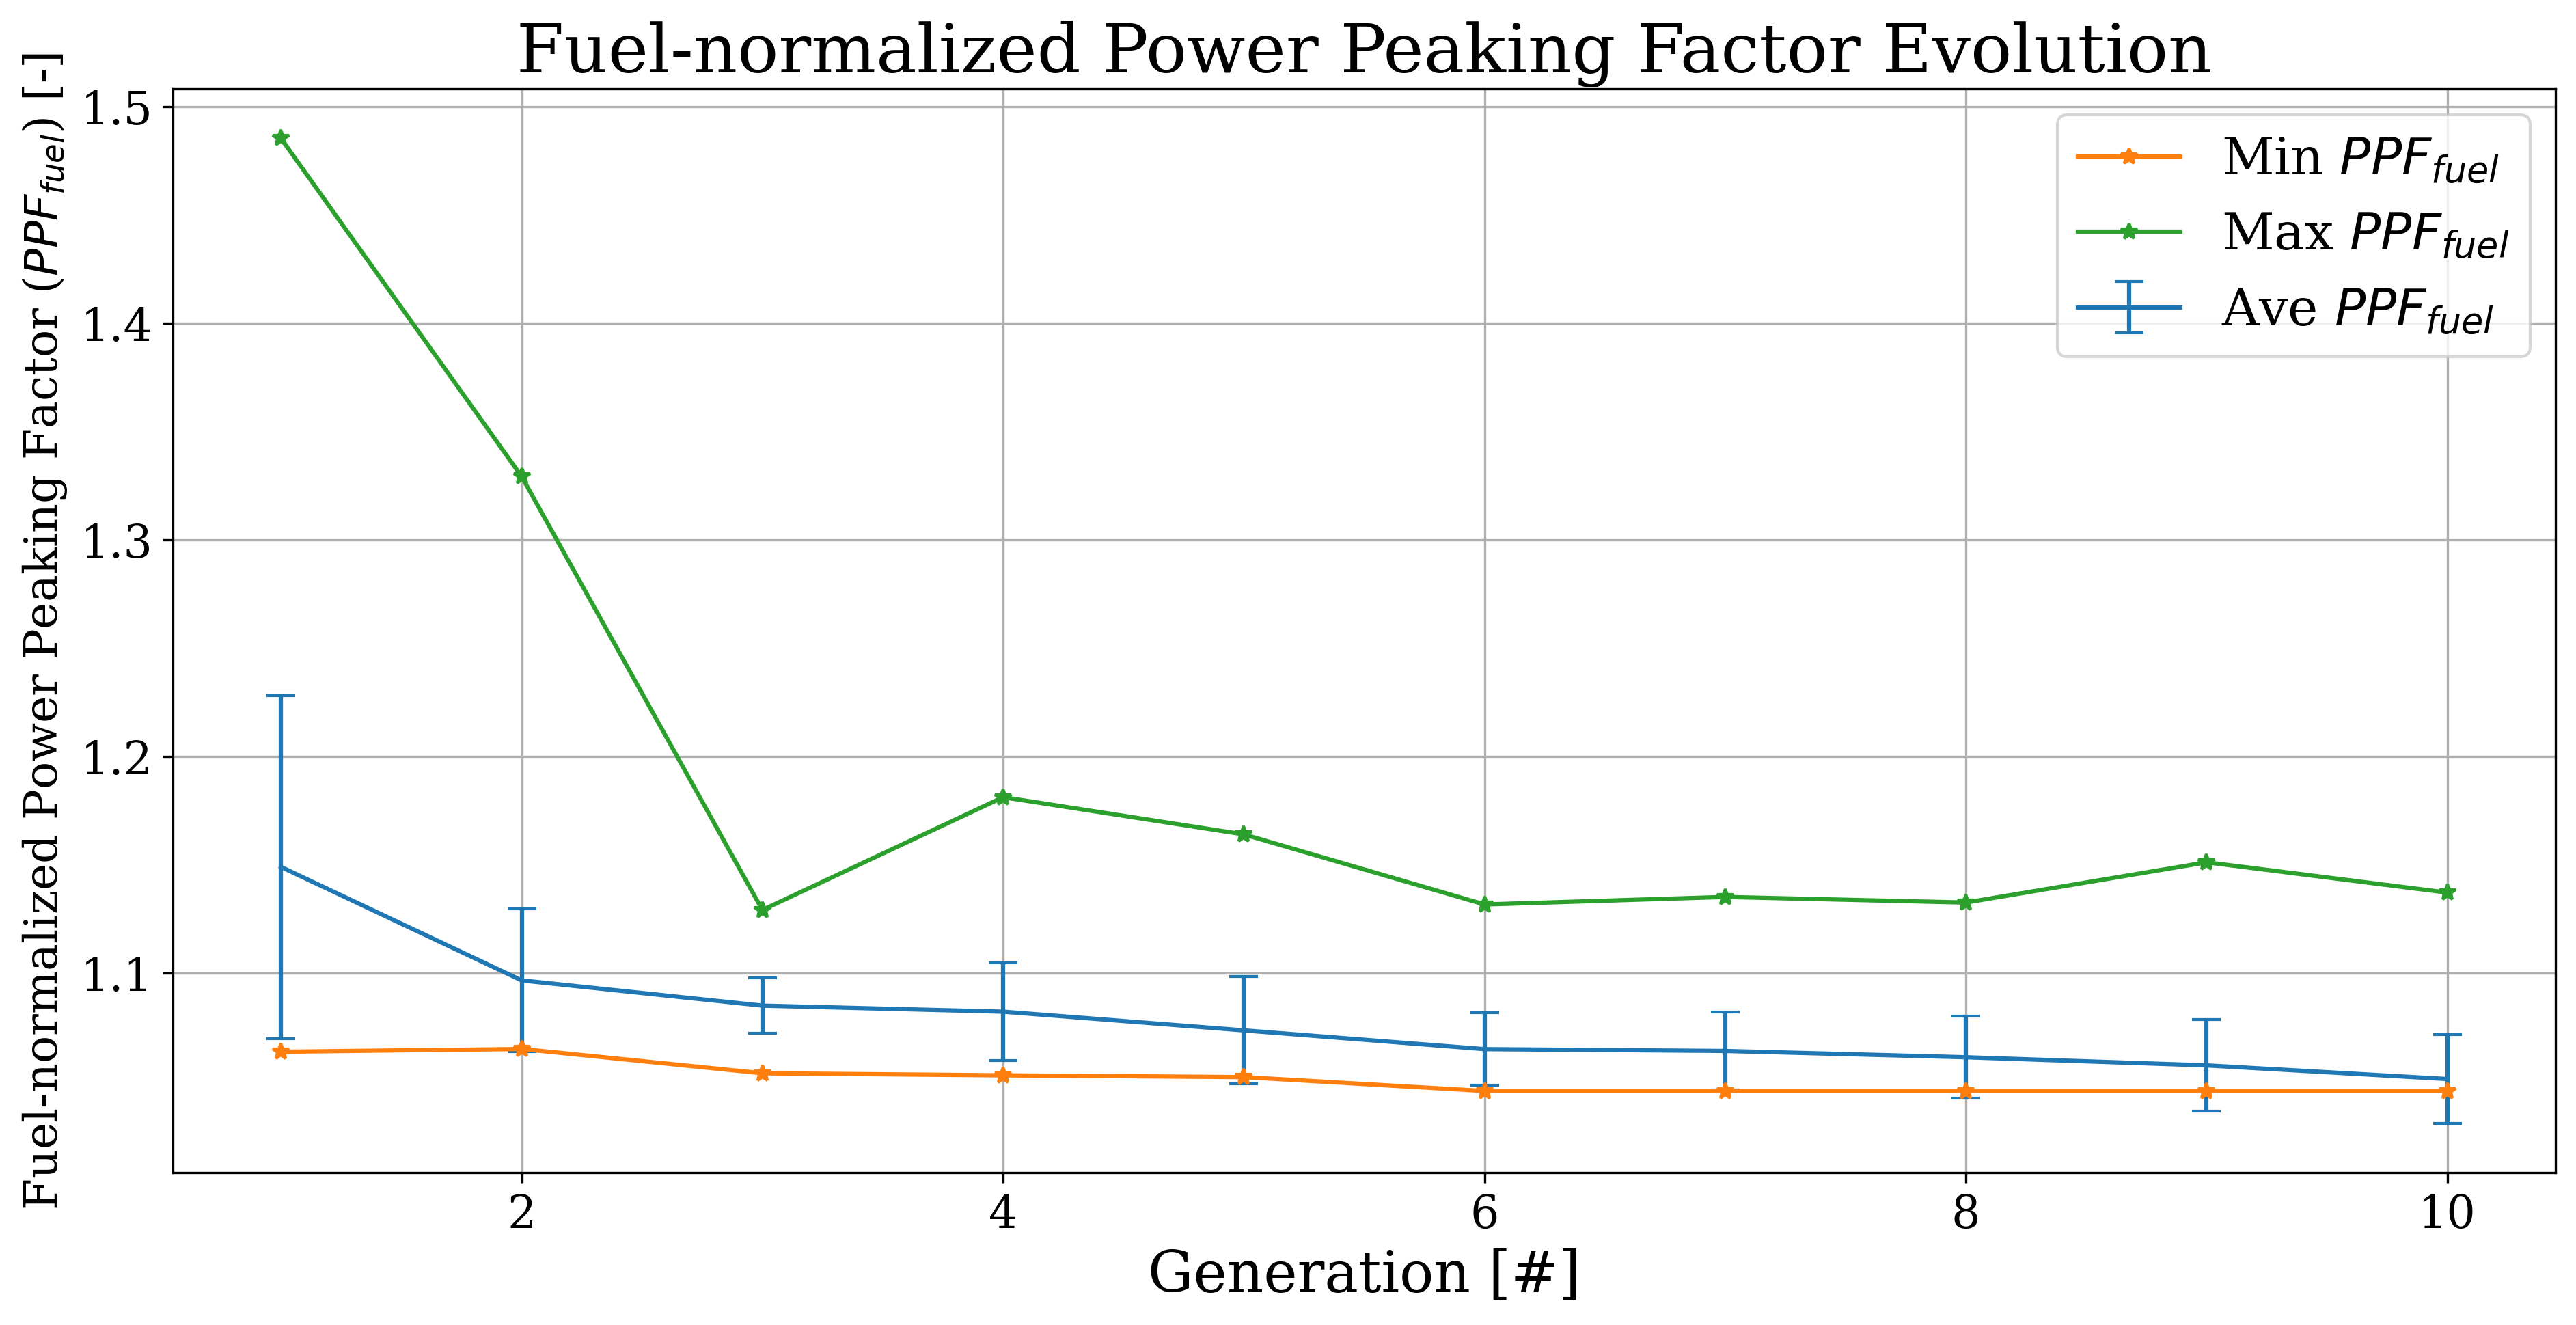
\includegraphics[width=\linewidth]{slab-obj-1-ppf-evol.png}
        \caption{Minimum, average, and maximum evolution of normalized power 
        peaking factor in AHTR slab.}
        \label{fig:slab-obj-1-ppf-evol} 
    \end{subfigure}
    \begin{subfigure}{\textwidth}
        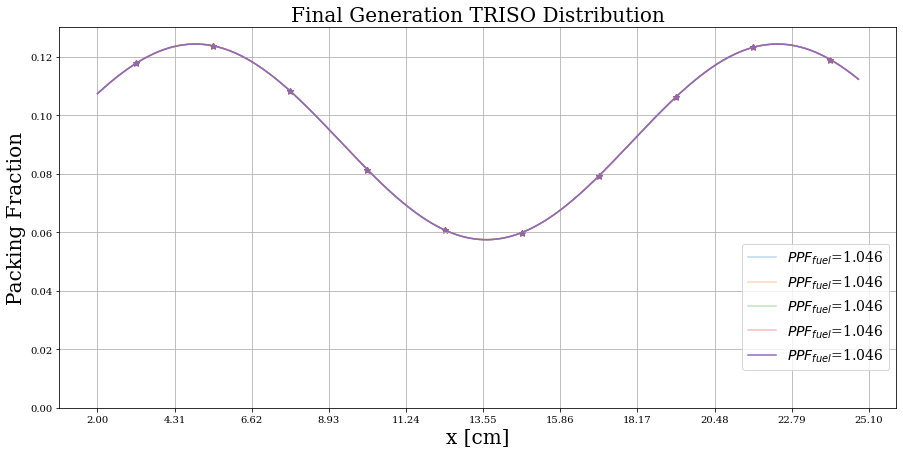
\includegraphics[width=\linewidth]{slab-obj-1-ppf-final.png}
        \caption{TRISO particle distribution for the 5 individuals with the 
        lowest normalized power peaking factor in AHTR slab at generation 9.}
        \label{fig:slab-obj-1-ppf-final} 
    \end{subfigure}
    \caption{ROLLO single-objective optimization to minimize normalized power 
    peaking factor in the slab. Input parameters varied: TRISO particle distribution.}
    \label{fig:slab-obj-1-ppf}
\end{figure}

\subsection{Multi-Objective Optimization}